\documentclass[11pt]{article}
\usepackage[margin=1in]{geometry}
\usepackage{amsmath}
\usepackage{amssymb}
\usepackage{setspace}
\usepackage{graphicx}

\usepackage{color}
\definecolor{deepblue}{rgb}{0,0,0.5}
\definecolor{deepred}{rgb}{0.6,0,0}
\definecolor{deepgreen}{rgb}{0,0.5,0}
\usepackage{listings}

\DeclareFixedFont{\ttb}{T1}{txtt}{bx}{n}{12} % for bold
\DeclareFixedFont{\ttm}{T1}{txtt}{m}{n}{12}  % for normal

% Python style for highlighting
\newcommand\pythonstyle{\lstset{
    language=Python,
    basicstyle=\ttm,
    otherkeywords={self},             % Add keywords here
    keywordstyle=\ttb\color{deepblue},
    emphstyle=\ttb\color{deepred},    % Custom highlighting style
    stringstyle=\color{deepgreen},
    frame=tb,                         % Any extra options here
    showstringspaces=false            % 
}}


% Python environment
\lstnewenvironment{python}[1][]
{
    \pythonstyle
    \lstset{#1}
}
{}

    

\begin{document}

\title{ECE 4750 Lab 1: Iterative Integer Multiplier}
\author{Akshay Dongaonkar (akd54) \& Avinash Navada (abn44) \& Vivek Gaddam (vrg22)}
\maketitle

\section{Introduction}

In many programming algorithms, multiplication is a key step in driving the algorithm towards completion. 
Many digital signal processing algorithms spend most of their time multiplying values. 
Given our media heavy, highly connected Internet of Things (IoT), more signals will need to be processed.
Therefore, we have synthesized an iterative multiplier that supports the mul instruction as defined in the PARCv1 Instruction Set Architecture (ISA).
Eventually, this multiplier will be a module in a fully synthesizable multicore processor.

We fully implemented two designs of an iterative multiplier: the base design is a fixed latency, 34 cycle iterative multiplier, while the alternative design is a variable latency iterative multiplier with bounds of 3 to 34 cycles.
While we do not expect much additional overhead on clock frequency in our alternative design,
we expect a significant increase in area and energy. Running our array of unit tests on both designs reveals that the variable design consumes far less clock cycles than does the base design (8.88 cycles/multiplication (alternative design) vs. 34 cycles/multiplication (base)).

We also scale down our hardware use in the variable design and determine that the associated performance downgrade on the same unit tests (to 9.1 cycles/multiplication) is still far superior to the base design. We expect the alternative design to be used over the base in most implementations and potential applications while still meeting modern technology constraints (focus on energy, large die sizes, etc).
  


\section{Project Management}

Given our group's various skill levels, we assigned Avinash to be verification lead, Vivek to be the architect, and Akshay to be the design lead.
Our initial project roadmap was fairly aggressive and required us to be finished by Wednesday, September $10^{th}$.
The intial Gantt Chart is shown in Figure~\ref{fig:gantt}. The actual roadmap is shown as a separate Gantt Chart (Figure~\ref{fig:gantt_actual}).

The breakdown of work follows:
Vivek implemented most of the baseline design and some of the alternate design in Verilog. 
Avinash implemented some of the alternate design and created our testing suite for Lab 1.
Akshay came up with the designs for the alternate design and wrote most of the writeup.
Akshay helped debug the Verilog code.
Vivek corrected the majority of errors in the RTL code.

Implementation of the RTL code progressed fairly smoothly with the exception of a few logical errors that were somewhat difficult to catch.
Vivek completed the baseline design while Avinash finished the directed test cases. We then tested the baseline design with these tests until it passed. This was one milestone in our agile development approach. Similarly, Akshay, Vivek, and Avinash completed the alternate design while Avinash finished the random test cases and added datasets for evaluation. After this was done, we spent a lot of time debugging the entire functionality of each design individually. We relied on the variety of tests in the testing suite to provide verification for this lab.

Some lessons learned from this lab were how to use tools such as GTKWave and line tracing to catch logic errors. 
Another idea for testing in future assignments is unit tests for the functionality of major modules within our implementation in addition to end-to-end tests of our overall implementation.

\section{Baseline Design}

The baseline design works on the following interface: 
given a 64 bit message containing our operands, a clock signal,
and required signals to conform to the val/rdy microprotocol,
output the lower 32 bits of the multiplication to your consumer.
This interface is shown in Figure~\ref{fig:model}.
Our algorithm for computing the multiplication is as follows.
If the least significant bit (lsb) of the second operand (call it $b$) is 1, add it to an accumulator.
Then, shift your first operand (call it $a$) left by one bit and the second operand to the right logically by one bit.
This is the first algorithm we are taught when we learn to multiply and is a good baseline for comparison because of the fact that a shift by one bit takes one cycle, making the design conceptually simple.
The pseudocode for this is shown in Figure~\ref{fig:code}. 

Our implementation follows the structure of this pseudo-code very closely.
We have three registers, one each for $a$, $b$, and $result$ (our accumulator).
We have 2 shifters, one logical left shifter and one logical right shifter. 
We have an equivalent multiplexor for the clause that adds to our accumulator if the lsb of $b$ is $1$.

However, the control logic and the data flow are not implemented as a monolithic design.
Instead, we implement a \textit{control-datapath split.}
The control module sends control signals to the datapath module, altering the flow of data into the registers.
This occurs when we are accepting new values into our operand registers,
writing/not-writing partial sums to $result$, and outputing a computed value.
The datapath module sends the lsb of $b$ to the control module so it can compute the appropriate dataflow.
The datapath is shown in Figure~\ref{fig:datapath}.
The lsb is directly used to determine whether to partially sum into $result$, a direct mapping to the pseudocode.

As seen from the pseudocode, there is no escape from the \verb+for+ loop.
Therefore, this implementation \textbf{must} take at least 32 cycles.
In fact, our implementation takes 34 cycles, as we have one cycle to accept data and one cycle to state we are done.
The state machine capturing this logic is shown in Figure~\ref{fig:BaseFSM}. 
This implementation, therefore, does exploit patterns in the underlying data.
In the most extreme case where $b$ is zero, the hardware checks every bit of $b$ and decides 32 times not to add to $result$.
We should reduce that down to one decision not to write to $result$.

While modularity was used in taking advantage of structures (such as shifters, registers, and adders) that were individually verified for correctness, we could have also used hierarchy. Notice that each register has a multiplexor in front of it directing output.
We could have wrapped that structure into a module and reused it three times. 
This would have allowed us to test incrementally and unit-by-unit.
Instead, we were forced to rely on end-to-end testing and test all functionality at once. This may have contributed to us not sooner catching RTL bugs.
Nevertheless, our use of encapsulation (by way of the val/rdy microprotocol) was a major feature of our design.

\section{Alternative Design}

The primary downside to our baseline implementation is the large latency in computing the product.
We propose several alternative designs and attempt to increase performance.
Since we cannot use concepts of indirection or caching, we might consider pipelineing our multiplier.
We could also consider exploiting the underlying structure of our operands to increase performance.
There are multiple ways to exploit structure in our operands; we will attempt to exploit structure in two ways.
First, we will roll over consecutive zeros by shifting more than 1 bit if possible.
Second, we will reduce the granularity of how many zeros we shift over to powers of two, as this reduces hardware costs
while still increasing performance over the fixed latency multiplier.
Both of these techniques exploit the \textit{regularity} in our input operands.

Let us first consider pipelining our multiplier, which seems to be applicable given the linear FSM used for the base design.
We can create stages between every state transition and have our val/rdy microprotocol mediate flow through the pipeline.
However, consider the hardware required. We need $34 \times 3 = 102$ registers, $34 \times 4 = 136$ two way multiplexors,
and $34$ logical left and right shifters.
This does not include the $34$ full adders we need. 
The cost of this design is enormous!
Additionally, this design only achieves high throughput if we get repeated multiplications.
Consider single cycle processors.
This design will add exactly zero improvement in those processors, as we cannot pipeline instructions. 
Also, since we are assuming we are going to get instructions from a canonical C program, this design seems impractical.

Instead, we can exploit the structure of the 32 bit operands we get.
We are likely to have some repeated set of zeros of length $n$ in our second operand.
Our algorithm in these cases does nothing to our result register, wasting $n$ cycles.
So, we will instead shift $n$ bits, saving us $n-1$ cycles in our computation.
We need one cycle to actually determine that there are $n$ bits we can skip.
Our state machine for this logic is shown in Figure~\ref{fig:AltFSM}.
We implement this change using the \verb+casez+ construct.
If there are multiple zeros in the lsb, we increment our counter by $n-1$ and shift by the appropriate amount.
So, if there is a zero in $b$, we shift 32 bits and spend only one cycle in the calc stage.
Therefore, our total overhead is 3 cycles: one for IDLE, one for CALC, and one for DONE.
If the $b$ operand is all ones, we take our usual 34 cycles.
That provides our range of multiply cycles we can take.

An advantage to this design is that the datapath gets modified only slightly.
We only add one more control signal to our shifters, and the lone status signal from the base design (the lsb of $b$) is now expanded to the full 32 bits of $b$.
In other words, \textbf{the datapath components for the alternative design are the same as for the base design (Figure~\ref{fig:datapath})}. 
This allowed us to rapidly implement the alternative design.

However, instead of shifting by $n$ bits, let us shift by powers of two.
This allows us to reduce the number of cases we need to check from 32 to 6.
This is a five-fold reduction in hardware! As mentioned in the introduction, this hardware reduction comes with little performance loss, and thus may be more appropriate in applications with technology constraints. 


\section{Testing Strategy}

The base and alternative designs were tested using the provided test harness, to which were added additional directed and random test cases.

The directed and random test cases were made to cover all types of possible inputs, including (decimal) zeros and ones, small and large numbers, positive and negative numbers, numbers with masked lower/middle bits, and combinations of these. The magnitude of the inputs was also varied considerably from 0 to 32 bits (even though the bit width of all the inputs is 32). Furthermore, test source/sink delays were also added to random tests to test the val/rdy microprotocol. A summary of all the different types of test cases is given in the table below.

\begin{center}
\begin{table}[h]
\begin{tabular}{|c | c | c|}
\hline
\textbf{Test Case}                    & \textbf{Test Case}                   & \textbf{Test Case}               \\
\hline
$\times$ of 0, 1, and $-1$            & small $(+) \times (+)$               & small $(-) \times (+)$           \\
small $(-) \times (+)$                & small $(-) \times (-)$               & large $(+) \times (+)$           \\
large $(+) \times (-)$                & large $(-) \times (+)$               & large $(-) \times (-)$           \\
$\times$ with low bits msk            & $\times$ with mid bits mks           & sparse $(+/-) \times (+/-)$      \\
dense  $(+/-) \times (+/-)$           & RS $\times$ RS                       & RS $\times$ with RD              \\
RL $\times$ RS                        & RL $\times$ RL with RD               & RS $\times$ RS with low bits msk \\
RS $\times$ RS with low bits msk w/RD & RL $\times$ RL with mid bits msk     &                                  \\
\hline                                                 
\end{tabular}
\caption{RS = Random Small, RL = Random Large, RD = Random Delays, msk = masked} 
\end{table}
\end{center}

At first only the functional model and base design worked correctly with these unit tests, while the alternative design failed most of them. At this point, we also used line traces and GTKWave to do more granular testing to ensure outputs were actually being generated and at the expected times. 

Ultimately both the base and alternative designs, as well as the functional model, worked correctly with all test cases. Although the tests were comprehensive and were developed in accordance with the increasing complexity of the control and datapath modules, we could have targeted the control and datapath modules separately with specific tests to ensure correct functionality before incorporating them together. However, this lab was simple enough for the test suite we wrote to be more than sufficient, especially since development of the baseline design was aided by comparison with the GCD model from Tutorial 3. 


\section{Evaluations and Conclusion}

As soon as the base and alternative designs were completed, the next step was to test the performance of the models. In order to achieve this, the simulator harness was built and run (using the given random dataset of small numbers) to generate the total number of cycles and the average number of cycles per transaction for the base and alternative designs. To expand on this, we added three more random datasets to the simulator harness to check the performance of the designs with different inputs: large numbers, low bits masked, and middle bits masked. The results of the simulator for each dataset and design are summarized in the table below.

\begin{table}[h]
\begin{tabular} {|l | r  | r | r | r|}

\hline
\textbf{Design}    & \textbf{DS: SI} & \textbf{DS: LI} & \textbf{DS: LB masked} & \textbf{DS: MB masked} \\
\hline
Baseline:    Total Cycles                 & 1751.00                        & 1751.00                        & 1751.00                 & 1751.00    \\
Baseline:    Avg. Cycles / Transaction    & 35.02                          & 35.02                          & 35.02                   & 35.02   \\
Alternative: Total Cycles                 & 444.00                         & 783.00                         & 666.00                  & 574.00     \\
Alternative: Avg. Cycles / Transaction    & 8.88                           & 15.66                          & 13.32                   & 11.48   \\
Alternative-Powers of 2:	Total Cycles  & 455						       & 817
& 723					  & 654
Alternative-Powers of 2:    Avg. Cycles / Transaction     & 9.1			   & 16.34
& 14.46					  & 13.08
\hline                    
\end{tabular}
\caption{Baseline v. Alternative Design Performance. DS = Dataset. SI = Small Inputs. LI = Large Inputs. LB = Low Bits. MB = Middle Bits.}
\end{table}


From the above table, we can see that the baseline design performs the same for all datasets, which is to be expected since it is a fixed-latency design. However, the alternative design performs far better than the baseline design for all input datasets as it capitalizes on inputs with consecutive zeroes to reduce latency. Interestingly, the alternative design performed better for the small inputs dataset than it did for the large inputs dataset, perhaps due to the large inputs dataset containing less consecutive zeroes and relatively denser inputs. It also performed better for the masked datasets than it did for the large inputs dataset due to the guaranteed presence of consecutive zeroes. The "powers of 2" alternative design (that only capitalized on numbers of consecutive zeroes that are powers of 2) did better than the baseline design but only slightly worse than the alternative design as expected since it didn't account for numbers of consecutive zeroes that aren't powers of 3 (1, 3, 5, 6, etc.). 

One area of improvement we considered but couldn't implement due to time constraints was capitalizing on consecutive ones in negative numbers. The idea was to convert negative inputs to their positive equivalents by flipping the bits and adding 1, multiplying the positive numbers together, and finally converting the product back to its negative equivalent. By converting the inputs to positive numbers, we can use the alternative design to capitalize on the consecutive zeroes (it doesn't work with consecutive ones). 
The possible alternative implementations discussed in the alternative design section could be used to further reduce latency and improve performance, especially by taking advantage of data-level parallelism even more. 


\begin{figure}[b]
\centering
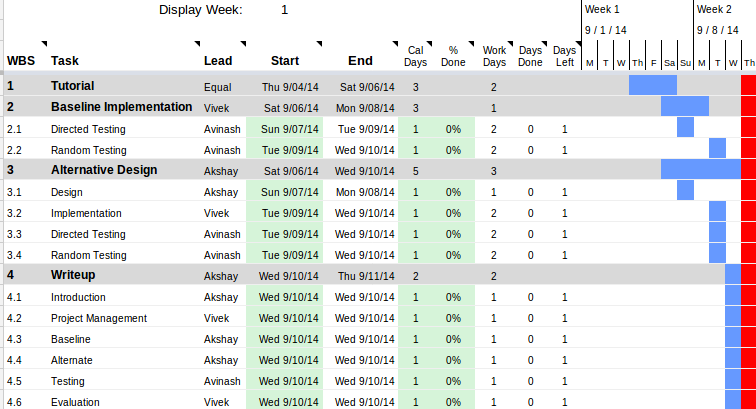
\includegraphics[scale=0.5]{gantt}
\caption{The initial Gantt chart postulating progress}
\label{fig:gantt}
\end{figure}

\begin{figure}[b]
\centering
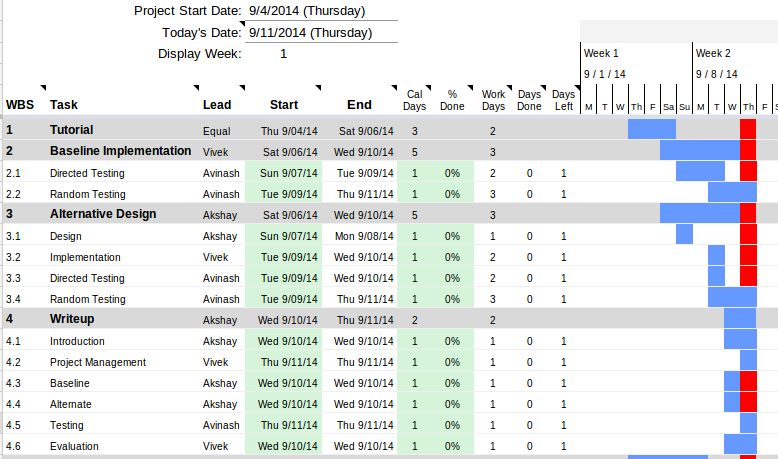
\includegraphics[scale=0.5]{gantt_actual}
\caption{Our actual progress on the lab}
\label{fig:gantt_actual}
\end{figure}

\begin{figure}[b]
\centering
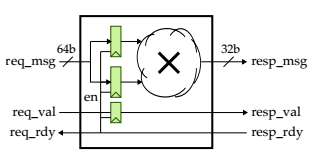
\includegraphics[scale=0.5]{FLmodel}
\caption{Interface for our model. Notice that req/resp,val/rdy signals are part of the val/rdy microprotocol}
\label{fig:model}
\end{figure}

\begin{figure}[b]
\centering
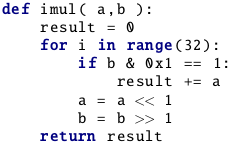
\includegraphics[scale=0.9]{imul}
\caption{Pseudocode for our baseline multiply algorithm}
\label{fig:code}
\end{figure}

\begin{figure}[b]
\centering
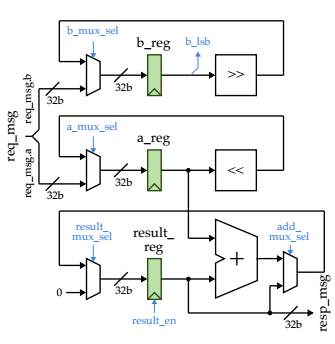
\includegraphics[scale=0.6]{Datapath}
\caption{Datapath Diagram. Again, the structure mimics the pseudocode.}
\label{fig:datapath}
\end{figure}

\begin{figure}[b]
\centering
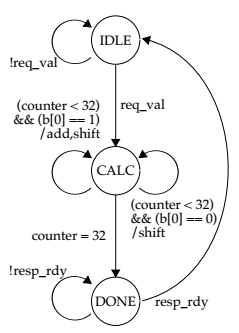
\includegraphics[scale=0.6]{BaseFSM}
\caption{FSM capturing control logic.}
\label{fig:BaseFSM}
\end{figure}

\begin{figure}[b]
\centering
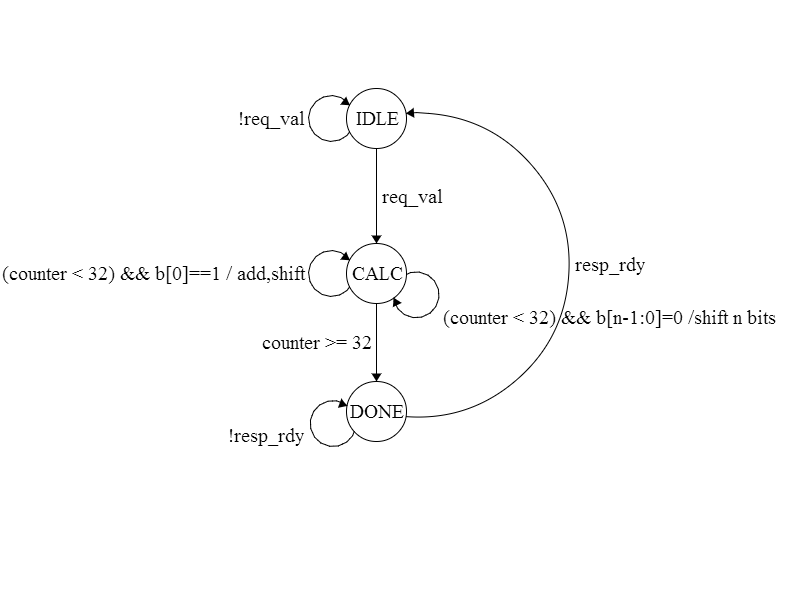
\includegraphics[scale=0.6]{AltFSM}
\caption{FSM capturing control logic for the alternative design.}
\label{fig:AltFSM}
\end{figure}




\end{document}
